% \appendix
% \newpage
\appendix
\section{Extended Background of Reinforcement Learning in LLMs}
\label{app:background_rl}

Reinforcement Learning (RL) enables large language models to improve through interaction and reward feedback. The general RL objective maximizes the expected reward over sampled responses:
\begin{equation}
    J(\theta) = \mathbb{E}_{x \sim \mathcal{D},\, y \sim \pi_\theta(\cdot \mid x)} \left[ R(x, y) \right],
\end{equation}
where \( \pi_\theta \) is the model policy, \( x \) is the input prompt, \( y \) is the generated output, and \( R(x, y) \) is a scalar reward assessing response quality.

A widely adopted method for RL fine-tuning is Proximal Policy Optimization (PPO)~\citep{ppo}, which stabilizes training by clipping the likelihood ratio between the new and old policies. The ratio is defined as:
\begin{equation}
    \rho_t(\theta) = \frac{\pi_\theta(y_t \mid x_t)}{\pi_{\theta_{\text{old}}}(y_t \mid x_t)}.
\end{equation}
The PPO objective minimizes over the clipped surrogate advantage:
\begin{equation}
    J_{\text{PPO}}(\theta) = \mathbb{E}_t \left[ \min\left( \rho_t A_t, \hat{\rho}_t A_t \right) - \beta D_{\mathrm{KL}} \right],
\end{equation}
where \( \hat{\rho}_t = \text{clip}(\rho_t, 1 - \epsilon, 1 + \epsilon) \), and \( A_t \) is the advantage function estimating how much better \( y_t \) is than the baseline under prompt \( x_t \).

For advantage estimation, Generalized Advantage Estimation (GAE)~\citep{schulman2015GAE} is often used:
\begin{equation}
    A_t^{\mathrm{GAE}(\gamma, \lambda)} = \sum_{l=0}^{\infty} (\gamma \lambda)^l \delta_{t+l}, \quad \text{with} \quad \delta_t = r_t + \gamma V(x_{t+1}) - V(x_t),
\end{equation}
where \( (\gamma, \lambda) \) trade off bias and variance.

More recently, DeepSeekMath \citep{deepseekmath} and DeepSeek-R1 \citep{deepseekr1} adopts Group Relative Policy Optimization (GRPO), a RL method that samples a set of outputs \( \{y_i\}_{i=1}^G \) for each prompt \( x \), and optimizes:
\begin{equation}
    J_{\text{GRPO}}(\theta) = \mathbb{E}_{x, \{y_i\}} \left[ J_{\text{group}}(\theta) \right],
\end{equation}
with
\begin{equation}
    J_{\text{group}}(\theta) = \frac{1}{G} \sum_{i=1}^G \min\left( \rho_i A_i, \hat{\rho}_i A_i \right) - \beta D_{\mathrm{KL}},
\end{equation}
where the advantage \( A_i \) is computed using a reward-normalized baseline:
\begin{equation}
    A_i = \frac{r_i - \text{mean}(\{r_j\})}{\text{std}(\{r_j\})}.
\end{equation}
This avoids dependency on value networks and uses rule-based or environment-specific rewards \( r_i \), making it well-suited for reasoning tasks where explicit heuristics can guide learning. GRPO has shown to induce emergent multi-step reasoning behavior across domains.


\section{Details on the Theoretical Analysis on Repetition Pattern}
\label{sec:app-repetition-theory}

We provide a detailed proof on how peaked, low-entropy output distribution from RL training \citep{cui2025entropymechanismreinforcementlearning, yue2025doesreinforcementlearningreally} can lead to high repetition in model multi-turn behavior.

\paragraph{Preliminaries.} Let $q(y \mid x)$ denote the model's output distribution given input $x$. We introduce the following definitions:

\begin{definition}[Collision Probability]
The collision probability of $q(y \mid x)$ is defined as:
\begin{equation}
\mathrm{Coll}(q) := \sum_y q(y \mid x)^2.
\end{equation}
This is the probability that two i.i.d.\ samples from $q$ yield the same answer: $\Pr[A_i = A_j] = \mathrm{Coll}(q)$.
\end{definition}

\begin{definition}[Entropy]
The Shannon entropy of $q(y \mid x)$ is:
\[
\mathcal{H}(q) := -\sum_y q(y \mid x) \log q(y \mid x).
\]
Lower entropy corresponds to a more peaked distribution.
\end{definition}

\begin{definition}[Expected Number of Duplicate Pairs]
Given $k$ i.i.d.\ samples $\{A_1, \dots, A_k\} \sim q(\cdot \mid x)$, the expected number of duplicate pairs is:
\[
\mathbb{E}[\mathrm{DupPairs}] = \binom{k}{2} \cdot \mathrm{Coll}(q).
\]
\end{definition}

\paragraph{Repetition Under Sequential Sampling.}
\begin{proposition}
\label{prop:collision-entropy}
Let $A_1, \dots, A_k \sim q(\cdot \mid x)$ be sampled sequentially.
Since single-turn RL does not guarantee any multi-turn capability, we simplify the assumption that the policy is static and does not update based on prior turns, i.e., the answer at each turn $t$ is sampled from the same fixed distribution $q(\cdot | x)$. The probability of generating a duplicate answer is the collision probability, which is lower-bounded by:
\[
\Pr[A_i = A_j] \ge \exp(-\mathcal{H}(q)),
\]
where $\mathcal{H}(q)$ denotes the Shannon entropy of the base distribution $q(\cdot \mid x)$.
\end{proposition}


\begin{proof}
Let \( Y \sim q(\cdot \mid x) \), and define the collision probability as:
\[
\mathrm{Coll}(q) = \mathbb{P}[A_i = A_j] = \sum_y q(y)^2 = \mathbb{E}_{Y \sim q}[q(Y)].
\]
By Jensen’s inequality applied to the concave function \( \log \), we have:
\[
\log \mathbb{E}_{Y}[q(Y)] \ge \mathbb{E}_{Y}[\log q(Y)] = -\mathcal{H}(q),
\]
which implies:
\[
\mathrm{Coll}(q) \ge \exp(-\mathcal{H}(q)).
\]
\end{proof}

\begin{remark}[On the Tightness of the Bound]
The lower bound $\mathrm{Coll}(q) \ge \exp(-\mathcal{H}(q))$ is tight in the following cases:
\begin{itemize}
    \item When $q$ is uniform on a support of size $n$, i.e., $q(y) = 1/n$, then $\mathcal{H}(q) = \log n$ and $\mathrm{Coll}(q) = 1/n$, achieving equality.
    \item When $q$ is a delta distribution (i.e., concentrated on one point), then $\mathcal{H}(q) = 0$ and $\mathrm{Coll}(q) = 1$.
\end{itemize}
We assume $\log q(y)$ is only computed where $q(y) > 0$, so the result still holds for distributions with zero-probability points.

A tighter bound can be obtained using the Rényi–Shannon inequality:
\[
\mathrm{Coll}(q) = e^{ -\mathcal{H}(q) - D_{\mathrm{KL}}(q \parallel u)},
\]
where $u$ is the uniform distribution on the support of $q$. Our stated bound omits the KL divergence for simplicity and interpretability.
\end{remark}

\noindent
This demonstrates that a low-entropy model is mathematically guaranteed to have a higher floor for its repetition rate. Thus, for a static agent that does not learn from feedback, repetition is not an accidental bug but a predictable outcome of the low-entropy distributions created by standard RL.

\section{Theoretical Analysis on Advantages of Sequential Policies}
\label{app:theory-ufo}
We model multi-turn reasoning as a finite-horizon Markov Decision Process (MDP), where the state at step \( t \) is given by
\[
s_t = (q, a_1, f_1, \dots, a_{t-1}, f_{t-1}),
\]
with input question \( q \), previous answers \( a_i \), and corresponding feedback \( f_i \). 

We represent policies as functions \( \pi_t(a \mid s_t) \) that produce an action \( a \) based on the interaction history \( s_t \). In our setting, the \textit{single-turn RL} paradigm corresponds to a \textbf{parallel policy}, where the model samples multiple answers independently from a fixed distribution \( \pi(a \mid q) \) without conditioning on feedback. In contrast, our \textit{UFO} (Unary Feedback as Observation) operates as a \textbf{sequential policy}, where the action at each step is conditioned on the full history and thus can adapt dynamically.

We formalize the distinction as follows:
\begin{itemize}
    \item \textbf{Parallel policies} \( \pi \in \Pi_{\text{par}} \): sample answers i.i.d.\ from a fixed policy \( \pi(a \mid q) \), without using feedback.
    \item \textbf{Sequential policies} \( \pi \in \Pi_{\text{seq}} \): choose actions based on the full state \( s_t \), enabling feedback-driven refinement.
\end{itemize}

Every parallel policy is a special case of a sequential policy that ignores interaction history. Formally, for any \( \pi(a \mid q) \), we can construct \( \pi_t(a \mid s_t) = \pi(a \mid q) \) for all \( t \), implying
\[
\Pi_{\text{par}} \subseteq \Pi_{\text{seq}}.
\]
Since \( \Pi_{\text{par}} \subseteq \Pi_{\text{seq}} \), we immediately have:
\[
\max_{\pi \in \Pi_{\text{seq}}} \mathbb{E}[\mathrm{Succ}@k] \ge \max_{\pi \in \Pi_{\text{par}}} \mathbb{E}[\mathrm{Succ}@k],
\]
where \(\mathrm{Succ}@k\) denotes the probability of producing a correct answer within \( k \) attempts.

Let \( p \) denote the success probability under a parallel policy. Then:
\[
\mathbb{P}_{\text{par}}[\text{success in } k \text{ turns}] = 1 - (1 - p)^k.
\]
For a sequential policy, let \( p'_t \) be the conditional success probability at step \( t \), which may depend on the state \( s_t \). The success probability is:
\[
\mathbb{P}_{\text{seq}}[\text{success in } k \text{ turns}] = 1 - \prod_{t=1}^k (1 - p'_t), \quad \text{where } p'_t \ge p.
\]
Sequential policies can eliminate previously failed answers by maintaining a rejection set \( \mathcal{H}_t \subset \mathcal{A} \) and enforcing:
\[
\pi_t(a \mid s_t) = 0 \quad \text{for all } a \in \mathcal{H}_t.
\]
This behavior approximates sampling without replacement and yields increasing conditional success rates:
\[
p'_t = \frac{p}{1 - \sum_{i=1}^{t-1} p_i} > p.
\]
Therefore, sequential policies such as UFO improve \(\mathrm{Succ}@k\) by adaptively avoiding prior failure modes. This formalizes the theoretical advantage of feedback-aware reasoning strategies over static single-turn RL.

\section{Detailed Evaluation under Multi-round Settings}

\begin{figure}[t]
    \centering
    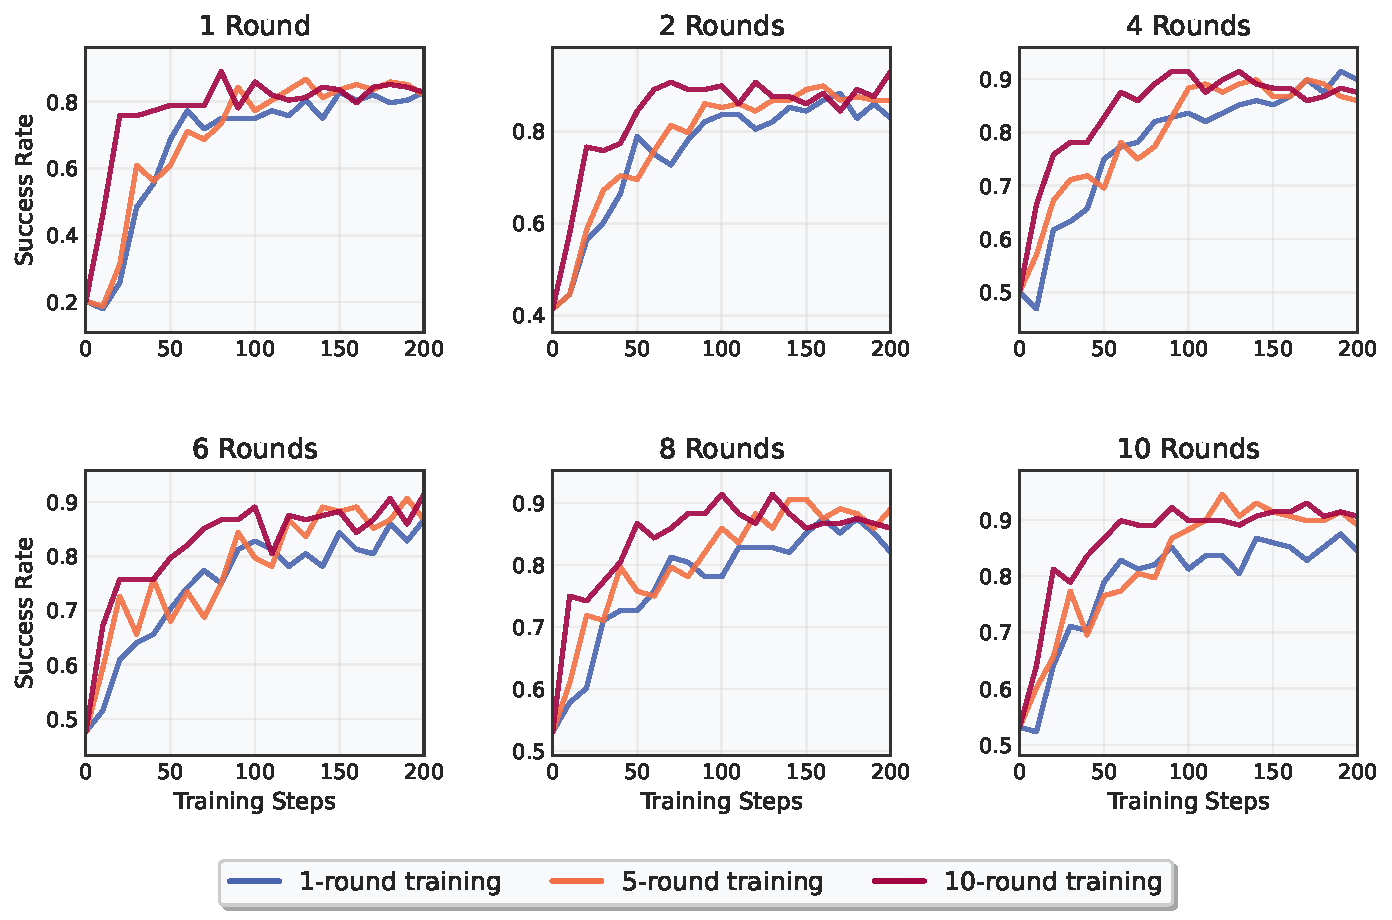
\includegraphics[width=0.98\linewidth]{figures/validation_rounds_comparison.pdf}
    \caption{\textbf{Performance across different evaluation round settings.} Each subplot shows the success rate evaluated at $r$ rounds. While all methods perform similarly under 1-round evaluation, models trained with multi-round feedback (UFO) generalize significantly better to longer evaluation horizons.}
    \label{fig:enter-label}
\end{figure}

We illustrate a detailed analysis of how multi-round training improves generalization on long-horizon interactive reasoning. Figure~\ref{fig:enter-label} provides a comprehensive view of validation performance across all checkpoints, comparing models trained under 1-round, 5-round, and 10-round settings. Each curve represents evaluation success rates under a fixed number of evaluation rounds.

We observe that under 1-round evaluation (top-left), all training strategies achieve similar performance, suggesting that even single-turn training can suffice in this limited setting. However, as evaluation round count increases, the gap between single-round training and multi-round training becomes increasingly significant. In particular, models trained with 10-round UFO feedback consistently outperform the others under 6, 8, and 10-round evaluation, demonstrating more stable and generalizable behavior across turns.

These results support our core hypothesis: \textbf{unary feedback, when used as structured observation during training, enables better long-horizon generalization.} In contrast, models trained only with single-round interactions struggle to adapt to multi-turn dynamics, leading to degraded performance as the task horizon increases.

\section{Prompt Settings}
\subsection{Problem Solving Model Prompt}
We adopt a simple and structured prompt format for mathematical problem solving, following prior designs from~\citet{deepseekmath, qwen25}, with an extension to support multi-turn interactions. 
A key element of our prompt is the explicit \texttt{<think>} and \texttt{<answer>} separation, paired with an action budget (\texttt{Y}) and max length (\texttt{Z}). This guides the model to reason step-by-step while planning within a fixed turn horizon, improving controllability and alignment in multi-turn settings.
As shown in Box~\ref{box:prompt}, we present the prompt template used during training and evaluation.

\begin{tcolorbox}[breakable, colback=gray!2, colframe=black, boxrule=0.5pt, arc=2pt, width=\linewidth, title=Box 1: Model Prompt Template]
\refstepcounter{examplebox}\label{box:prompt}
\texttt{<|im\_start|>system\\
\{prompt\}\\
You're a helpful assistant.\\
<|im\_end|>\\
<|im\_start|>user\\
\{prompt\}\\
You are solving Math problems.\\
Turn X:\\
State:\\
(Question)\\
You have Y actions left. Always output: <think> [Your thoughts] </think> <answer> [your answer] </answer> with no extra text. Strictly follow this format. Max response length: Z words (tokens).\\
<|im\_end|>\\
<|im\_start|>assistant\\
... (This conversation pattern repeats for up to K turns) \\
<|im\_end|>
}\par
\end{tcolorbox}


\subsection{Feedback Provider Model Prompt}
We also present the prompt for the feedback provider that gives the problem-solving model more detailed feedback as follows.

\begin{tcolorbox}[breakable, colback=gray!2, colframe=black, boxrule=0.5pt, arc=2pt, width=\linewidth, title=Box 2: Tutor Prompt Template]
\refstepcounter{examplebox}\label{box:tutorprompt}
\texttt{<|im\_start|>system\\
You are a helpful math tutor.\\
<|im\_end|>\\
<|im\_start|>user\\
Problem: \{question\}\\
Student's answer: \{wrong\_answer\}\\
This answer is incorrect. Give a brief, encouraging hint (1--2 sentences) that helps the student reconsider their approach without revealing the correct answer. Focus on guiding them to check their work or think about the problem differently.\\
Response format: Just the hint, no extra formatting.\\
<|im\_end|>\\
<|im\_start|>assistant\\
...\\
<|im\_end|>}
\end{tcolorbox}

\subsection{TheoremQA Prompt Format}
The TheoremQA environment follows a similar prompting structure as the MMQ-Math, with an additional image token placed at the beginning of the question when a picture is present. This enables compatibility with multimodal pipelines, where the image is processed separately while the text prompt includes a placeholder token to signal its presence.

As shown in Box~\ref{box:theoremqa}, the image token \texttt{<image>} is placed on a new line above the question if an image is available.

\begin{tcolorbox}[breakable, colback=gray!2, colframe=black, boxrule=0.5pt, arc=2pt, width=\linewidth, title=Box 3: TheoremQA Prompt Template]
\refstepcounter{examplebox}\label{box:theoremqa}
\texttt{<|im\_start|>system\\
You're a helpful assistant.\\
<|im\_end|>\\
<|im\_start|>user\\
\{prompt\}\\
You are solving Math problems.\\
Turn X:\\
State:\\
<image>\\
+ (Question)\\
You have Y actions left. Always output: <think>[Your thoughts]</think><answer>[your answer]</answer> with no extra text. Strictly follow this format. Max response length: Z words (tokens).\\
<|im\_end|>\\
<|im\_start|>assistant\\
...\\
<|im\_end|>}
\end{tcolorbox}

\section{Model Evaluation Details}
\label{sec:model-detail}
We present the model used to evaluate answer repetition in Table~\ref{tab:hf-model-names}.

\begin{table}[t]
\centering
\caption{Hugging Face model names used in the unique answer ratio evaluation.}
\begin{tabular}{ll}
\toprule
\textbf{Method} & \textbf{Model (Hugging Face name)} \\
\midrule
DAPO & Qwen/Qwen2.5-32B \\
     & BytedTsinghua-SIA/DAPO-Qwen-32B \\
\midrule
Dr.\ GRPO & Qwen/Qwen2.5-Math-7B \\
          & sail/Qwen2.5-Math-7B-Oat-Zero \\
          & Qwen/Qwen2.5-Math-1.5B \\
          & sail/Qwen2.5-Math-1.5B-Oat-Zero \\
\midrule
GRPO & Qwen/Qwen2.5-0.5B \\
     & hkust-nlp/Qwen-2.5-0.5B-SimpleRL-Zoo\\
     & Qwen/Qwen2.5-1.5B \\
     & hkust-nlp/Qwen-2.5-1.5B-SimpleRL-Zoo \\
     & Qwen/Qwen2.5-7B \\
     & hkust-nlp/Qwen-2.5-7B-SimpleRL-Zoo \\
     & Qwen/Qwen2.5-14B \\
     & hkust-nlp/Qwen-2.5-14B-SimpleRL-Zoo \\
\midrule
PPO & Qwen/Qwen2.5-Math-7B \\
    & RLHFlow/Qwen2.5-7B-PPO-Zero \\
    & Qwen/Qwen2.5-3B-Instruct \\
    & LichengLiu03/Qwen2.5-3B-UFO \\
    
\bottomrule
\end{tabular}
\label{tab:hf-model-names}
\end{table}


\section{Case Analyses}

We investigate the impact of multi-turn reinforcement learning (RL) on large language models (LLMs) through a series of curated examples across distinct training stages. These case studies (shown in Boxes~\ref{box:case1}--\ref{box:case4}) highlight the evolving dynamics of exploration, convergence, and reasoning quality throughout training.


\subsection{Case 1: Pre-training Behavior}
Before any reinforcement learning, we observe the model’s default multi-turn reasoning behavior in a symbolic pattern-matching task (Box~\ref{box:case1}). The model is asked to recover a missing variable \(X\) from a repeating alphabetic value pattern, given partial information and a constraint on the sum of values in a specific word. In Turn 1, the model identifies the relevant positions in the word “numeric” and proposes an initial guess for \(X\). As feedback indicates the answer is incorrect, the model progressively refines its understanding: it attempts to align characters in the input word with their positions in the pattern and adjusts its value for \(X\).

Despite making several wrong guesses, the model demonstrates \textbf{adaptive behavior across turns}: it updates its assumptions, introduces new hypotheses, and makes meaningful structural progress (e.g., recognizing the 8-length cycle). However, it ultimately fails to reach the correct solution within the available steps. The case shows that \textbf{pretrained models already possess multi-step reflective capabilities and can utilize external feedback to revise their reasoning}, even without explicit training for multi-turn alignment. It suggest that reinforcement learning has the potential to further stabilize and guide emergent reasoning process toward convergence.


\subsection{Case 2: Post Single-turn RL}
After reinforcement learning with single-step reward feedback, the model demonstrates drastically different behavior from its pretrained counterpart (Box~\ref{box:case2}). When tasked with identifying the variable \(X\) in a cyclic pattern-based word problem, the model immediately commits to a single interpretation. In Turn 1, it attempts a symbolic derivation by aligning the letter values of “numeric” with a fixed periodic pattern, then solving \(X - 3 = -1\). However, this derivation mistakenly assumes that the letters in “numeric” correspond to the first 7 elements of the pattern without justifying the mapping. More notably, this exact sequence of logic and answer is \textbf{repeated identically} in Turns 2 through 5.

\textbf{The case reveals that single-turn RL induces brittle, overconfident behavior}: once the model settles on a trajectory during initial inference, it does not reconsider alternative hypotheses or respond meaningfully to corrective feedback. The reward optimization has led to collapse in exploration, as each turn simply replays the same incorrect reasoning with no adaptation. In contrast to the pretraining stage, where the model at least attempts different strategies, this behavior illustrates a major drawback of single-step reward supervision: it teaches the model what to say once, but not how to revise when it’s wrong.

\subsection{Case 3: Success Adaptation to Feedback Through Multi-turn RL with UFO }
This example illustrates the effectiveness of multi-turn reinforcement learning (Box~\ref{box:case3}). The model is prompted to determine the sum of all positive integers \(n\) for which \(\frac{n + 18}{n}\) is an integer. In Turn 1, it begins by simplifying the expression to \(1 + \frac{18}{n}\), and attempts a partial answer without listing all divisors. Upon receiving feedback, the model updates its understanding in Turn 2 by enumerating all positive divisors of 18. By Turn 3, it completes the reasoning process by summing those divisors correctly, arriving at the correct final answer of 39.

The case shows a successful case of multi-turn self-correction, where the model refines its reasoning incrementally in response to feedback. Each turn builds on the previous one: the model first identifies the mathematical form, then retrieves the correct domain knowledge (divisors), and finally executes a complete and valid computation. Unlike single-turn RL, \textbf{the multi-turn reward structure encourages adaptive reasoning and gradual convergence.} The example shows that properly trained multi-turn agents can both reason correctly and update their behavior mid-trajectory in pursuit of a verifiable answer.


\subsection{Case 4: Reasoning Drift of Multi-turn RL with UFO}
We examine a failure trajectory under multi-turn reinforcement learning where the model arrives at the correct final answer through incorrect or misaligned reasoning. As shown in Box~\ref{box:case4}, the task is to find the value of \(X\) such that the matrix \(\begin{pmatrix} X & 3 \\ -1 & 7 \end{pmatrix}\) has an inverse consistent with the given answer “17.” In the initial turn, the model misinterprets the problem structure by assuming that the matrix inverse itself is the scalar 17, and raises a structural objection. In the next turn, it shifts to a more plausible interpretation where 17 is assumed to be the determinant. This leads to the formulation of the correct equation \(7X + 3 = 17\), though the value of \(X\) is still miscalculated at that stage.

By the third turn, the model correctly solves for \(X = 2\), but then presents a flawed expression for the inverse matrix, misapplying the standard inversion formula for \(2 \times 2\) matrices. Despite producing the right numerical solution, the trajectory contains conceptual errors related to matrix algebra, including an incorrect cofactor layout. This case highlights a form of reasoning drift: \textbf{while the final output aligns with the ground truth, the intermediate steps do not constitute a logically valid derivation.} Such behavior reveals a potential failure of reward design in multi-turn RL, where correctness of the answer is reinforced even in the absence of faithful reasoning.



\begin{table}[t]
\centering
\caption{Comparison of multi-turn reasoning behaviors across training stages.}
\begin{tabular}{@{}llllll@{}}
\toprule
\textbf{Case} & \textbf{Stage} & \textbf{Exploration} & \textbf{Convergence} & \textbf{Reasoning Quality} & \textbf{Failure Mode} \\
\midrule
1 & Pre-RL           & High      & No    & Incomplete         & Early guessing \\
2 & Single-turn RL   & None      & No    & Repetitive         & Overfitting     \\
3 & Multi-turn RL   & Moderate  & Yes   & Correct & aligned              \\
4 & Multi-turn RL   & Moderate  & Yes   & Incorrect          & Reasoning drift \\
\bottomrule
\end{tabular}
\label{tab:cases_summary}
\end{table}

To summarize (as in Table~\ref{tab:cases_summary}), multi-turn RL with UFO improves convergence and stabilizes reasoning, but naive reward design can still lead to misalignment between thought and outcome. It highlights the need for evaluation frameworks to go beyond final answer correctness and explicitly assess reasoning integrity throughout the trajectory.


\begin{tcolorbox}[breakable, colback=gray!2, colframe=black, boxrule=0.5pt, arc=2pt, width=\linewidth, title=Box 4: Multi-Turn Rollout before training]
\refstepcounter{examplebox}\label{box:case1}
\textbf{Turn 1:} \\
\textbf{State:}
The letters of the alphabet are given numeric values based on the two conditions below.

$\bullet$  Only the numeric values of $-2,$ $-1,$ $0,$ $1$ and $2$ are used.

$\bullet$  Starting with A and going through Z, a numeric value is assigned to each letter according to the following pattern: $$
1, 2, X, 0, -1, -2, -1, 0, 1, 2, 1, 0, -1, -2, -1, 0,\ldots
$$

Two complete cycles of the pattern are shown above. The letter A has a value of $1,$ B has a value of $2,$ F has a value of $-2$ and Z has a value of $2$. The sum of the numeric values of the letters in the word ``numeric" is -1. What is the value of unknown variable X?
You have 10 actions left. Always output: \texttt{<think>} [Your thoughts] \texttt{<think>} \texttt{<answer>} [your answer] \texttt{<answer>} with no extra text. Strictly follow this format. Max response length: 100 words (tokens). \\
\textbf{Output:} \\
\texttt{<think>}First, let's identify the positions of each letter in the word ``numeric" based on the pattern provided. We know the values of A, B, F, and Z. We need to determine the value of X and then find the values of N, M, E, and C to sum up to -1.\texttt{</think>} \\
\texttt{<answer>}X = 2\texttt{</answer>} \\
Reward: 0.0

\vspace{4pt}
\textbf{Turn 2:} \\
\textbf{State:}
Incorrect. Please try agin.
You have 3 actions left. Always output: \texttt{<think>} [Your thoughts] \texttt{<think>} \texttt{<answer>} [your answer] \texttt{<answer>} with no extra text. Strictly follow this format. Max response length: 100 words (tokens). \\
\textbf{Output:} \\
\texttt{<think>}Given the incorrect answer, let's re-examine the pattern and the values assigned to each letter. The word ``numeric" has the letters N, U, M, B, E, I, C. From the provided pattern, we know the values of A, B, F, and Z. To find the value of X, we need to identify the value for N and then determine the pattern for subsequent letters.\texttt{</think>} \\
\texttt{<answer>}X = 0\texttt{</answer>} \\
Reward: 0.0

\vspace{4pt}
\textbf{Turn 3:} \\
\textbf{State:}
Incorrect. Please try agin.
You have 2 actions left. Always output: \texttt{<think>} [Your thoughts] \texttt{<think>} \texttt{<answer>} [your answer] \texttt{<answer>} with no extra text. Strictly follow this format. Max response length: 100 words (tokens). \\
\textbf{Output:} \\
\texttt{<think>}Given the incorrect answer, let's re-evaluate the pattern and the values assigned to each letter in the word ``numeric". The values for A, B, F, and Z are known. The pattern seems to repeat every 8 letters, and the values cycle through 1, 2, X, 0, -1, -2, -1, 0. We need to determine the value of X such that the sum of the values of the letters in ``numeric" equals -1.\texttt{</think>} \\
\texttt{<answer>}X = -1\texttt{</answer>} \\
Reward: 0.0

\vspace{4pt}
\textbf{Turn 4:} \\
\textbf{State:}
Incorrect. Please try agin.
You have 1 actions left. Always output: \texttt{<think>} [Your thoughts] \texttt{<think>} \texttt{<answer>} [your answer] \texttt{<answer>} with no extra text. Strictly follow this format. Max response length: 100 words (tokens). \\
\textbf{Output:} \\
\texttt{<think>}Given the incorrect answer, let's re-examine the pattern and the values assigned to each letter in the word ``numeric". The values for A, B, F, and Z are known, and the pattern seems to repeat every 8 letters with values 1, 2, X, 0, -1, -2, -1, 0. To find the value of X such that the sum of the values of the letters in ``numeric" equals -1, we need to assign values to N, U, M, B, E, I, C and ensure their sum is -1\texttt{</think>} \\
\texttt{<answer>}X = 1\texttt{</answer>} \\
Reward: 0.0 \\

\vspace{4pt}
\textbf{Turn 5:} \\
\textbf{State:}
Incorrect. Please try agin.
You have 0 actions left. Always output: \texttt{<think>} [Your thoughts] \texttt{<think>} \texttt{<answer>} [your answer] \texttt{<answer>} with no extra text. Strictly follow this format. Max response length: 100 words (tokens). \\
\textbf{Output:} \\
\texttt{<think>}Given the incorrect answer, let's re-examine the pattern and the values assigned to each letter in the word ``numeric". The values for A, B, F, and Z are known, and the pattern seems to repeat every 8 letters with values 1, 2, X, 0, -1, -2, -1, 0. To find the value of X such that the sum of the values of the letters in ``numeric" equals -1, we need to assign values to N, U, M, B, E, I, C and ensure their sum is -1.\texttt{</think>} \\
\texttt{<answer>}X = -1\texttt{</answer>} \\
Reward: 0.0
\end{tcolorbox}


\begin{tcolorbox}[breakable, colback=gray!2, colframe=black, boxrule=0.5pt, arc=2pt, width=\linewidth, title=Box 5: Model rollout after single-turn RL training]
\refstepcounter{examplebox}\label{box:case2}
\textbf{Turn 1:} \\
\textbf{State:}
The letters of the alphabet are given numeric values based on the two conditions below.

$\bullet$  Only the numeric values of $-2,$ $-1,$ $0,$ $1$ and $2$ are used.

$\bullet$  Starting with A and going through Z, a numeric value is assigned to each letter according to the following pattern: $$
1, 2, X, 0, -1, -2, -1, 0, 1, 2, 1, 0, -1, -2, -1, 0,\ldots
$$

Two complete cycles of the pattern are shown above. The letter A has a value of $1,$ B has a value of $2,$ F has a value of $-2$ and Z has a value of $2$. The sum of the numeric values of the letters in the word ``numeric" is -1. What is the value of unknown variable X?
You have 10 actions left. Always output: \texttt{<think>} [Your thoughts] \texttt{<think>} \texttt{<answer>} [your answer] \texttt{<answer>} with no extra text. Strictly follow this format. Max response length: 100 words (tokens). \\
\textbf{Output:} \\
\texttt{<think>}For the word ``numeric", the values of the letters are as follows: N has a value of 1, U has a value of 2, M has a value of 0, E has a value of -1, R has a value of -2, I has a value of -1, C has a value of 1. The sum of these values is \(1 + 2 + 0 - 1 - 2 - 1 + 1 = 0\), which contradicts the given sum of -1. However, we can re-evaluate the pattern and the values. The pattern repeats every 16 letters, and the values repeat as well. The word ``numeric" consists of 7 letters, so we need to find the sum of the first 7 values in the pattern: \(1, 2, X, 0, -1, -2, -1\). We know the sum of these values is -1. So, we have \(1 + 2 + X + 0 - 1 - 2 - 1 = -1\), which simplifies to \(X - 3 = -1\), and thus \(X = 2\).\texttt{</think>} \\
\texttt{<answer>}2\texttt{</answer>} \\
Reward: 0.0

\vspace{4pt}
\textbf{Turn 2:} \\
\textbf{State:}
Incorrect. Please try agin.
You have 3 actions left. Always output: \texttt{<think>} [Your thoughts] \texttt{<think>} \texttt{<answer>} [your answer] \texttt{<answer>} with no extra text. Strictly follow this format. Max response length: 100 words (tokens). \\
\textbf{Output:} \\
\texttt{<think>}For the word ``numeric", the values of the letters are as follows: N has a value of 1, U has a value of 2, M has a value of 0, E has a value of -1, R has a value of -2, I has a value of -1, C has a value of 1. The sum of these values is \(1 + 2 + 0 - 1 - 2 - 1 + 1 = 0\), which contradicts the given sum of -1. The pattern repeats every 16 letters, and the values repeat as \(1, 2, X, 0, -1, -2, -1, 0, 1, 2, 1, 0, -1, -2, -1, 0\). For the word ``numeric", the values are \(1, 2, X, 0, -1, -2, -1\). The sum of these values is \(1 + 2 + X + 0 - 1 - 2 - 1 = -1\), which simplifies to \(X - 3 = -1\), and thus \(X = 2\).\texttt{</think>} \\
\texttt{<answer>}2\texttt{</answer>} \\
Reward: 0.0

\vspace{4pt}
\textbf{Turn 3:} \\
\textbf{State:}
Incorrect. Please try agin.
You have 2 actions left. Always output: \texttt{<think>} [Your thoughts] \texttt{<think>} \texttt{<answer>} [your answer] \texttt{<answer>} with no extra text. Strictly follow this format. Max response length: 100 words (tokens). \\
\textbf{Output:} \\
\texttt{<think>}For the word ``numeric", the values of the letters are as follows: N has a value of 1, U has a value of 2, M has a value of 0, E has a value of -1, R has a value of -2, I has a value of -1, C has a value of 1. The sum of these values is \(1 + 2 + 0 - 1 - 2 - 1 + 1 = 0\), which contradicts the given sum of -1. The pattern repeats every 16 letters, and the values repeat as \(1, 2, X, 0, -1, -2, -1, 0, 1, 2, 1, 0, -1, -2, -1, 0\). For the word ``numeric", the values are \(1, 2, X, 0, -1, -2, -1\). The sum of these values is \(1 + 2 + X + 0 - 1 - 2 - 1 = -1\), which simplifies to \(X - 3 = -1\), and thus \(X = 2\).\texttt{</think>} \\
\texttt{<answer>}2\texttt{</answer>} \\
Reward: 0.0

\vspace{4pt}
\textbf{Turn 4:} \\
\textbf{State:}
Incorrect. Please try agin.
You have 1 actions left. Always output: \texttt{<think>} [Your thoughts] \texttt{<think>} \texttt{<answer>} [your answer] \texttt{<answer>} with no extra text. Strictly follow this format. Max response length: 100 words (tokens). \\
\textbf{Output:} \\
\texttt{<think>}For the word ``numeric", the values of the letters are as follows: N has a value of 1, U has a value of 2, M has a value of 0, E has a value of -1, R has a value of -2, I has a value of -1, C has a value of 1. The sum of these values is \(1 + 2 + 0 - 1 - 2 - 1 + 1 = 0\), which contradicts the given sum of -1. The pattern repeats every 16 letters, and the values repeat as \(1, 2, X, 0, -1, -2, -1, 0, 1, 2, 1, 0, -1, -2, -1, 0\). For the word ``numeric", the values are \(1, 2, X, 0, -1, -2, -1\). The sum of these values is \(1 + 2 + X + 0 - 1 - 2 - 1 = -1\), which simplifies to \(X - 3 = -1\), and thus \(X = 2\).\texttt{</think>} \\
\texttt{<answer>}2\texttt{</answer>} \\
Reward: 0.0 \\
\vspace{4pt}
\textbf{Turn 5:} \\
\textbf{State:}
Incorrect. Please try agin.
You have 0 actions left. Always output: \texttt{<think>} [Your thoughts] \texttt{<think>} \texttt{<answer>} [your answer] \texttt{<answer>} with no extra text. Strictly follow this format. Max response length: 100 words (tokens). \\
\textbf{Output:} \\
\texttt{<think>}For the word ``numeric", the values of the letters are as follows: N has a value of 1, U has a value of 2, M has a value of 0, E has a value of -1, R has a value of -2, I has a value of -1, C has a value of 1. The sum of these values is \(1 + 2 + 0 - 1 - 2 - 1 + 1 = 0\), which contradicts the given sum of -1. The pattern repeats every 16 letters, and the values repeat as \(1, 2, X, 0, -1, -2, -1, 0, 1, 2, 1, 0, -1, -2, -1, 0\). For the word ``numeric", the values are \(1, 2, X, 0, -1, -2, -1\). The sum of these values is \(1 + 2 + X + 0 - 1 - 2 - 1 = -1\), which simplifies to \(X - 3 = -1\), and thus \(X = 2\).\texttt{</think>} \\
\texttt{<answer>}2\texttt{</answer>} \\
Reward: 0.0
\end{tcolorbox}




\begin{tcolorbox}[breakable, colback=gray!2, colframe=black, boxrule=0.5pt, arc=2pt, width=\linewidth, title=Box 6: Model rollout after multi-turn RL training with UFO (Success Case)]
\refstepcounter{examplebox}\label{box:case3}
\textbf{Turn 1:} \\
\textbf{State:} \\
Determine the sum of all positive integer values of \(n\) such that \(\frac{n+18}{n}\) is an integer. \\
You have 10 actions left. Always output: \texttt{<think>} [Your thoughts] \texttt{</think>} \texttt{<answer>} [your answer] \texttt{</answer>} with no extra text. Strictly follow this format. Max response length: 100 words. \\
\textbf{Output:} \\
\texttt{<think>}First, I need to understand when \(\frac{n+18}{n}\) is an integer. This fraction can be simplified to \(1 + \frac{18}{n}\). For this to be an integer, \(n\) must be a divisor of 18.\texttt{</think>} \\
\texttt{<answer>}18 and 1 (since \(1 + \frac{18}{18} = 2\) and \(1 + \frac{18}{1} = 19\) are integers)\texttt{</answer>} \\
Reward: 0.0

\vspace{4pt}
\textbf{Turn 2:} \\
\textbf{State:} \\
Incorrect. Please think again. \\
You have 9 actions left. \\
\textbf{Output:} \\
\texttt{<think>}Given \(\frac{n+18}{n}\) is an integer, we have \(1 + \frac{18}{n}\) as an integer. This means \(n\) must be a divisor of 18. The positive divisors of 18 are 1, 2, 3, 6, 9, and 18. I need to verify which of these values make the expression an integer.\texttt{</think>} \\
\texttt{<answer>}1, 2, 3, 6, 9, 18\texttt{</answer>} \\
Reward: 0.0

\vspace{4pt}
\textbf{Turn 3:} \\
\textbf{State:} \\
Incorrect. Please think again. \\
You have 8 actions left. \\
\textbf{Output:} \\
\texttt{<think>}Upon reviewing, I realize the divisors of 18 are 1, 2, 3, 6, 9, and 18. For each of these values, \(1 + \frac{18}{n}\) is indeed an integer. Therefore, the sum of all positive integer values of \(n\) is \(1 + 2 + 3 + 6 + 9 + 18 = 39\).\texttt{</think>} \\
\texttt{<answer>}39\texttt{</answer>} \\
Reward: 0.25
\end{tcolorbox}

\begin{tcolorbox}[breakable, colback=gray!2, colframe=black, boxrule=0.5pt, arc=2pt, width=\linewidth, title=Box 7: Model rollout after multi-turn RL training with UFO (Failure Case)]
\refstepcounter{examplebox}\label{box:case4}
\textbf{Turn 1:} \\
\textbf{State:} \\
Find the inverse of the matrix
\[
\begin{pmatrix} X & 3 \\ -1 & 7 \end{pmatrix}.
\]
If the inverse does not exist, then enter the zero matrix. The answer is 17. What is the value of unknown variable \(X\)? \\
You have 10 actions left. Always output: \texttt{<think>} [Your thoughts] \texttt{</think>} \texttt{<answer>} [your answer] \texttt{</answer>} with no extra text. Strictly follow this format. Max response length: 100 words. \\
\textbf{Output:} \\
\texttt{<think>}Since the inverse of a matrix is given as 17, and the matrix provided is 2x2, the inverse should be a 2x2 matrix. However, the given inverse of 17 does not align with the structure of a 2x2 matrix. The problem might have a mistake in the provided inverse value or the matrix structure.\texttt{</think>} \\
\texttt{<answer>}There is an inconsistency in the problem statement. The given inverse of 17 does not match the structure of a 2x2 matrix inverse.\texttt{</answer>} \\
Reward: 0.0

\vspace{4pt}
\textbf{Turn 2:} \\
\textbf{State:} \\
Incorrect. Please think again. \\
You have 9 actions left. \\
\textbf{Output:} \\
\texttt{<think>}Given the inverse of the matrix is provided as 17, which does not fit the expected format of a 2x2 matrix inverse (which should be a 2x2 matrix), it seems there might be a misunderstanding. However, since the problem statement specifies the inverse as 17, and considering the structure of the matrix, it implies the inverse is a scalar value. For a 2x2 matrix \(\begin{pmatrix} a & b \\ c & d \end{pmatrix}\), the inverse is \(\frac{1}{ad-bc}\begin{pmatrix} d & -b \\ -c & a \end{pmatrix}\). If the inverse is simply 17, it suggests \(ad - bc = 17\). Given the matrix \(\begin{pmatrix} X & 3 \\ -1 & 7 \end{pmatrix}\), \(ad - bc = X \cdot 7 - 3 \cdot (-1) = 7X + 3\). Thus, \(7X + 3 = 17\).\texttt{</think>} \\
\texttt{<answer>}7\texttt{</answer>} \\
Reward: 0.0

\vspace{4pt}
\textbf{Turn 3:} \\
\textbf{State:} \\
Incorrect. Please think again. \\
You have 8 actions left. \\
\textbf{Output:} \\
\texttt{<think>}Given the matrix \(\begin{pmatrix} X & 3 \\ -1 & 7 \end{pmatrix}\), the condition for the inverse to be a scalar 17 is \(7X + 3 = 17\). Solving for \(X\) gives \(7X = 14\), thus \(X = 2\). The inverse of the matrix should be \(\frac{1}{17}\begin{pmatrix} 7 & -3 \\ 1 & X \end{pmatrix}\), which simplifies to \(\begin{pmatrix} \frac{7}{17} & -\frac{3}{17} \\ \frac{1}{17} & 2 \end{pmatrix}\), not just 17.\texttt{</think>} \\
\texttt{<answer>}2\texttt{</answer>} \\
Reward: 0.25
\end{tcolorbox}
